
	\section{Теорема Бохнера о спектральном представлении ковариационной функции.}
	
	\textbf{Автор:} Смородина Жанна Викторовна, Б-01-006
	
 	\subsection{Введение.}

    \subsubsection{Вспомогательные определения.}
    
    \begin{definition}\label{smd_def_1} \textbf{Корреляционной функцией} случайного процесса $\xi(t)$ называется математическое ожидание произведения двух сечений случайного процесса в моменты времени $t_1, t_2$ :
    $$
     R_{\xi}\left(t_1, t_2\right)=M\left[\xi\left(t_1\right) \xi\left(t_2\right)\right]=  \int\limits_{-\infty}^{\infty} \int\limits_{-\infty}^{\infty} x_1 x_2 \  d \mu\left(x_1, t_1 ; x_2, t_2\right) .
    $$
    Она определяется двумерной функцией распределения $\mu\left(x_1, t_1 ; x_2, t_2\right)$. \newline Данную функцию также называют \textbf{функцией автокорреляции}.
    \end{definition}
    
  
    \begin{definition}\label{smd_def_2} \textbf{Ковариационная функция} случайного процесса - это математическое ожидание произведения центрированных сечений процесса в моменты времени $t_1, t_2$ :
    $$
    K_{\xi}\left(t_1, t_2\right)=\operatorname{cov}\left(\xi\left(t_1\right) \xi\left(t_2\right)\right) = M\left[\left(\xi\left(t_1\right)-m_{\xi}\left(t_1\right)\right)\left(\xi\left(t_2\right)-m_{\xi}\left(t_2\right)\right)\right] .
    $$
    
    Величину
    $$
    r_{\xi}\left(t_1, t_2\right)=\frac{K_{\xi}\left(t_1, t_2\right)}{\sqrt{D_{\xi}\left(t_1\right) D_{\xi}\left(t_2\right)}}=\frac{K_{\xi}\left(t_1, t_2\right)}{\sqrt{K_{\xi}\left(t_1, t_1\right) K_{\xi}\left(t_2, t_2\right)}}
    $$
    называют нормированной ковариационной функцией или \textbf{коэффициентом корреляции} случайного процесса.
    
    Очевидно, что при $t_1=t_2=t$ ковариационная функция совпадает с дисперсией случайного процесса: $K_{\xi}(t, t)=D_{\xi}(t)=$ $=\sigma_{\xi}^2(t)$.
    
    Для 2-ух случайных процессов $\xi(t)$ и $\eta(t)$ вводится понятие взаимной функции корреляции, или \textbf{функции кросскорреляции}:
    $$
    R_{\xi \eta}\left(t_1, t_2\right)=M\left[\xi\left(t_1\right) \eta\left(t_2\right)\right],
    $$
    а совместная корреляционная функция 2 случайных процессов определяется как матричная функция $\left(\begin{array}{cc}R_{\xi}\left(t_1, t_2\right) & R_{\xi \eta}\left(t_1, t_2\right) \\ R_{\eta \xi}\left(t_1, t_2\right) & R_\eta\left(t_1, t_2\right)\end{array}\right)$.
	\end{definition}
    

    
    \begin{definition}\label{smd_def_3} Случайный процесс $\xi(t)$ называется \textbf{стационарным в узком смысле}, если для конечномерных функций распределения выполняется равенство
    \begin{equation}
            F\left(x_1, t_1 ; x_2, t_2 ; \ldots ; x_n, t_n\right)
    =F\left(x_1, t_1+\tau ; x_2, t_2+\tau ; \ldots ; x_n, t_n+\tau\right)
    \label{14.1}
    \end{equation}    
    $\forall \tau$ и $\forall n\in \mathbb{N}$, т.е. его конечномерное распределение инвариантно относительно сдвига всех моментов времени $t_i$, $i=\overline{1, n}$, на одну и ту же величину $\tau$.
     \newline При $n=1$ условие стационарности (\ref{14.1}) дает
    $$
    F\left(x_1, t_1\right)=F\left(x_1, t_1+\tau\right) .
    $$
    \end{definition}
    
    Полагая $\tau=-t_1$ $\  \left(F\left(x_1, t_1\right)=F\left(x_1, 0\right)\right) $, приходим к тому, что одномерное распределение стационарного процесса не зависит от времени и совпадает с распределением в момент времени $t=0$ $ \left(F\left(x_1, t_1\right)=F\left(x_1, 0\right)\right) $, а одномерное распределение определяет среднее значение и дисперсию случайного процесса. Следовательно, для стационарного в узком смысле случайного процесса среднее значение и дисперсия не зависят от времени:
    $$
        m_{\xi}(t)=m, \quad D_{\xi}(t)=\sigma^2 .
    $$

    При $n=2$ из условия стационарности следует
    $$
    F\left(x_1, t_1 ; x_2, t_2\right)=F\left(x_1, t_1+\tau ; x_2, t_2+\tau\right) .
x	    $$
    
    Полагая $\tau=-t_1$, получим: 
    $\ \  F\left(x_1, t_1 ; x_2, t_2\right)=F\left(x_1, x_2, t_2-t_1\right), $
    то есть двумерное распределение зависит лишь от разности моментов времени $t_2$ и $t_1$. Поэтому корреляционная функция стационарного в узком смысле случайного процесса зависит только от одного аргумента $t=t_2-t_1$.

    Стационарность в узком смысле означает, что все статистические характеристики процесса не подвергаются изменению при переносе оси времени. В частности, одномерное распределение не зависит от времени вообще. Процесс, стационарный в узком смысле, часто называют просто стационарным.


   \begin{definition}\label{smd_def_4} Случайный процесс $\xi(t)$ называется \textbf{стационарным в широком смысле}, если его среднее значение не зависит от времени:
    \begin{equation}
        m_{\xi}(t) = m ,
        \label{14.3}
    \end{equation}
    а корреляционная функция зависит лишь от разности аргументов:
    \begin{equation}
    R_{\xi}\left(t_1, t_2\right)=R_{\xi}\left(t_2-t_1\right) .
        \label{14.4}
    \end{equation}
	\end{definition}
    
    Очевидно, что из стационарности в узком смысле следует стационарность в широком смысле. Наоборот верно не всегда. Но для гауссовских случайных процессов верно и обратное утверждение.
    
    \begin{theorem}\label{smd_theor_1} \textit{Гауссовский процесс стационарный в широком смысле является стационарным и в узком смысле.}
    
    $\square$ $n$-мерная функция распределения такого процесса равна
    \begin{equation}
        \begin{gathered}
        F\left(x_1, t_1 ; x_2, t_2 ; \ldots ; x_n, t_n\right)=\frac{1}{(2 \pi)^{\frac{n}{2}} \sqrt{|K|}} \int\limits_{-\infty}^{x_1} \times \\
        \times \int\limits_{-\infty}^{x_2} \ldots \int\limits_{-\infty}^{x_n} 
        \exp \left\{-\frac{1}{2|K|} \sum_{i, j=1}^n\left[\left(y_i-a_i\right) K_{i j}\left(y_j-a_j\right)\right]\right\}  d y_1 d y_2 \dots d y_n , 
        \end{gathered}
        \label{14.5}
    \end{equation}
    где $a_i=M \xi\left(t_i\right), K=\parallel  K\left(t_i, t_j\right)\parallel  =\parallel  M\left[\left(\xi\left(t_i\right)-a_i\right)\left(\xi\left(t_j\right)-a_j\right)\right]\parallel  _{n \times n}$, \newline $i, j=\overline{1, n}, \ \  K_{i j} -$  алгебраическое дополнение элемента $K\left(t_i, t_j\right)$ матрицы $K$. 
    \end{theorem}

	\begin{proof}
    Для стационарного в широком смысле процесса, как следует из (\ref{14.3}), (\ref{14.4}):
    $$
    K\left(t_i, t_j\right)=K\left(t_i+\tau, t_j+\tau\right)=K\left(t_j-t_i\right) .
    $$
    Поэтому многомерная функция распределения (\ref{14.5}) зависит только от $n$ и $K\left(t_j-t_i\right):$
    $$
    F\left(x_1, t_1 ; x_2, t_2 ; \ldots ; x_n, t_n\right)=f\left(x_i, n, K\left(t_j-t_i\right)\right),\ \  i, j=\overline{1, n} .
    $$
    Теперь видно, что при переходе к моментам времени $t_i+\tau, \  i=\overline{1, n}$, функция распределения не изменится. 
    Таким образом, соотношение (\ref{14.1}) выполнено.
    \end{proof}

    Как сказано ранее, функцию корреляции стационарного в широком смысле случайного процесса можно рассматривать как функцию одного аргумента $R_{\xi}(t)$, которая для произвольного случайного процесса обладает следующими свойствами:
    
    a)  \begin{equation}
            R_{\xi}(0) \geq 0 ,
            \label{14.6}
        \end{equation}
        
    б)  \begin{equation}
            \left|R_{\xi}(t)\right| \leq R_{\xi}(0) ,
            \label{14.7}
        \end{equation}
        
    в) $R_{\xi}(t)$ является положительно определенной функцией, то есть:
    \begin{equation}
    \forall n,\ \  \forall z_1, z_2, \ldots, z_n \in \mathbb{C} \qquad    \sum_{i, j=1}^n R_{\xi}\left(t_i-t_j\right) z_i \bar{z}_j \geq 0 .
        \label{14.8}
    \end{equation}

    \begin{definition}\label{smd_def_5} Процессы $\xi(t)$ и $\eta(t)$ называются \textbf{стационарно связанными в узком смысле}, если их совместная конечномерная функция распределения любого порядка не зависит от положения начала отсчета времени, то есть 
   \newline  $ \forall \tau$ и $ \forall n, m \in\mathbb{N} $:
    $$
    \begin{aligned}
    & F\left(x_1, t_1 ; x_2, t_2 ; \ldots ; x_n, t_n ; y_1, \tau_1 ; y_2, \tau_2 ; \ldots ; y_m, \tau_m\right)= \\
    = & F\left(x_1, t_1+\tau ; x_2, t_2+\tau ; \ldots ; x_n, t_n+\tau\  y_1, \tau_1+\tau ; y_2, \tau_2+\tau ; \ldots ; y_m, \tau_m+\tau\right) \\
    \end{aligned}
    $$
    \end{definition}
    
    \begin{definition}\label{smd_def_6} Комплексный случайный процесс 
     $ \zeta(t)=\xi(t)+i \eta(t) $
    называется \textbf{стационарным в узком смысле}, если $\xi(t)$ и $\eta(t)$ являются стационарно связанными в узком смысле, т.е. его конечномерное распределение любого порядка $n$ удовлетворяет соотношению
    $$
    \begin{gathered}
    F_\zeta\left(x_1, t_1 ; x_2, t_2 ; \ldots ; x_n, t_n ; y_1, t_1 ; y_2, t_2 ; \ldots ; y_n, t_n\right)= \\
    =F_\zeta\left(x_1, t_1+\tau ; x_2, t_2+\tau ; \ldots ; x_n, t_n+\tau ; y_1, t_1+\tau ; y_2, t_2+\tau ; \ldots ; y_n, t_n+\tau\right) .
    \end{gathered}
    $$
    \end{definition}
    
    \begin{definition}\label{smd_def_7} Пусть $\zeta(t)$ - комплексный случайный процесс, такой, что 
    \newline $M \zeta^2(t)<\infty$. Он называется \textbf{стационарным в широком смысле}, если
    \begin{enumerate}
        \item $ M \zeta(t) = const $ ,
        \item $ R_\zeta\left(t_1, t_2\right) = M\left[\zeta\left(t_1\right) \overline{\zeta\left(t_2\right)}\right]=R_\zeta\left(t_2-t_1\right) $.
    \end{enumerate}
	\end{definition}
    
    \subsubsection{Теорема об обращении характеристической функции}

    Данная теорема позволяет находить ф.р. случайной величины, если известна ее характеристическая функция.
    
    \begin{definition}\label{smd_theor_2} Если $F_{\xi}(x)$ - ф.р. случайной величины $\xi,\ \  \varphi_{\xi}(t)$ - ее характеристическая функция, то для любых точек непрерывности $x$ и $y$ функции $F_{\xi}(x)$ выполнено:
    $$
    F_{\xi}(y)-F_{\xi}(x)=\lim _{\tau \rightarrow \infty} \frac{1}{2 \pi} \int\limits_{-\tau}^\tau\left(e^{-i t x}-e^{-i t y}\right) \varphi_{\xi}(t) \frac{1}{i t} d t .
    $$
    \end{definition}
 
    \begin{proof} 1) Пусть $F_{\xi}(x)-$ абсолютно непрерывная функция. В этом случае существует обратное преобразование Фурье:
    $$
    p_{\xi}(x)=\frac{1}{2 \pi} \int\limits_{-\infty}^{+\infty} e^{-i t x} \varphi_{\xi}(t) d t .
    $$
    Тогда, проинтегрировав обе стороны данного соотношения от $x$ до $y$, получим
    $$
    \begin{aligned}
    & F_{\xi}(y)-F_{\xi}(x)=\int\limits_x^y p_{\xi}(z) d z=\frac{1}{2 \pi} \int\limits_x^y \int\limits_{-\infty}^{+\infty} e^{-i t x} \varphi_{\xi}(t) d t d z= \\
    = & \frac{1}{2 \pi} \int\limits_{-\infty}^{+\infty} \varphi_{\xi}(t) \int\limits_x^y e^{-i t z} d z d t=\frac{1}{2 \pi} \int\limits_{-\infty}^{+\infty} \varphi_{\xi}(t) \frac{1}{i t}\left(e^{-i t x}-e^{-i t y}\right) d t .
    \end{aligned}
    $$
    
    2) Докажем теперь теорему в общем случае. Нужно показать, что
    $$
    \int\limits_x^y d F_{\xi}(z)=\lim _{\tau \rightarrow \infty} \frac{1}{2 \pi} \int\limits_{-\tau}^\tau\left(e^{-i t x}-e^{-i t y}\right) \varphi_{\xi}(t) \frac{d t}{i t} .
    $$
    В правой части этого соотношения имеем
    \begin{equation}
        \begin{gathered}
        \int\limits_{-\tau}^\tau\left(e^{-i t x}-e^{-i t y}\right) \int\limits_{-\infty}^{\infty} d F_{\xi}(z) \frac{d t}{i t}= \\
        =\int\limits_{-\infty}^{\infty} d F_{\xi}(z) \int\limits_{-\tau}^\tau\left(e^{i t(z-x)}-e^{i t(z-y)}\right) \frac{d t}{i t}= \\
        =\int\limits_{-\infty}^{\infty} d F_{\xi}(z) \int\limits_0^\tau\left(e^{i t(z-x)}-e^{i t(z-y)}+e^{-i t(z-y)}-e^{-i t(z-x)}\right) \frac{d t}{i t} .
        \end{gathered}
        \label{4.1}
    \end{equation}
    Рассмотрим отдельно внутренний интеграл, в который входит переменная $x$ :
    $$
    \begin{gathered}
    \int\limits_0^\tau\left(e^{i t(z-x)}-e^{-i t(z-x)}\right) \frac{d t}{i t}= \\
    =\int\limits_0^\tau[\cos (t(z-x))+i \sin (t(z-x))-\cos (t(z-x))+i \sin (t(z-x))] \frac{d t}{i t}= \\
    =2 \int\limits_0^\tau \sin (t(z-x)) \frac{d t}{t}=2 \int\limits_0^{\tau(z-x)} \frac{\sin u}{u} d u,
    \end{gathered}
    $$
    Правую часть выражения (\ref{4.1}) можно записать в виде
        $$
    \begin{gathered}
    2 \int\limits_{-\infty}^{\infty} d F_{\xi}(z)\left(\int\limits_0^{\tau(z-x)} \frac{\sin u}{u} d u-\int\limits_0^{\tau(z-y)} \frac{\sin u}{u} d u\right)= \\
    =2 \int\limits_{-\infty}^{\infty} d F_{\xi}(z) \int\limits_{\tau(z-y)}^{\tau(z-x)} \frac{\sin u}{u} d u .
    \end{gathered}
    $$
    Далее рассмотрим предел
    \begin{equation}
         \lim _{\tau \rightarrow \infty} \frac{1}{2 \pi} 2 \int\limits_{-\infty}^{\infty} d F_{\xi}(z) \int\limits_{\tau(z-y)}^{\tau(z-x)} \frac{\sin u}{u} d u .
         \label{4.2}
    \end{equation}
    
    Так как подынтегральное выражение равномерно ограничено, то можно изменять порядок интегрирования и обращения к пределу, т.е. выражение (\ref{4.2}) имеет следующий вид:
    $$
    \int\limits_{-\infty}^{\infty} d F_{\xi}(z) \lim _{\tau \rightarrow \infty} \frac{1}{\pi} \int\limits_{\tau(z-y)}^{\tau(z-x)} \frac{\sin u}{u} d u .
    $$
    Но по формуле Дирихле
    $$
    \lim _{\tau \rightarrow \infty} \frac{1}{\pi} \int\limits_{\tau(z-y)}^{\tau(z-x)} \frac{\sin u}{u} d u= \begin{cases}1, & x<z<y, \\ 0, & \text { в других случаях. }\end{cases}
    $$
    значит, выражение (\ref{4.2}) равно $F_{\xi}(y)-F_{\xi}(x)$. 
    \end{proof}

    Следствием из этой теоремы является \textit{\textbf{теорема единственности:}}
      \textit{Характеристическая функция СВ $\xi$ однозначно определяет ее функцию распределения.}

  
    \subsection{Теорема Бохнера и следствие из неё.}
    \subsubsection{Теорема Бохнера.}

  \begin{theorem}\label{smd_theor_3} \textit{Для функции $R(t)$, обладающей свойствами (\ref{14.6}) - (\ref{14.8}), существует неубывающая функция ограниченной вариации $F(\lambda)$ такая, что:}
    \begin{equation}
    R(t)=\int\limits_{-\infty}^{+\infty} e^{i \lambda t} d F(\lambda)
    \label{14.11}
    \end{equation}
	\end{theorem}
    
    \begin{proof}
    Пусть $z_i=e^{-i \lambda t_i}, i=1,2, \ldots$. Тогда из определения положительно определенной функции (\ref{14.8}) следует, что
    $$
    \sum_{i, j} R\left(t_i-t_j\right) e^{-i \lambda\left(t_i-t_j\right)} \geq 0 .
    $$
    
    Поэтому
    \begin{equation}
        g(\lambda, A)=\frac{1}{\sqrt{2 \pi} A} \int\limits_0^A \int\limits_0^A R(t-u) e^{-i \lambda(t-u)} d t d u \geq 0 \quad \forall A>0 .
        \label{14.12}
    \end{equation}

    Сделаем в интеграле (\ref{14.12}) замену переменных: $t-u=x,\ \  u=y$, тогда $x=t-y$. При этом область интегрирования $B$ перейдет в область интегрирования $C$, как показано на рисунке.

    \begin{center} 
        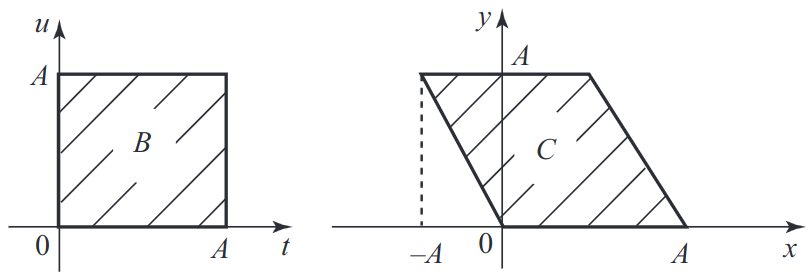
\includegraphics[width = \linewidth]{smd_jv_pic_1.png}
    \end{center}

    \begin{equation}
        \begin{aligned}
        g(\lambda, A) & = \frac{1}{\sqrt{2 \pi} A}\left[\int\limits_{-A-x}^0 \int\limits_0^A d y R(x) e^{-i \lambda x} d x+\int\limits_0^A \int\limits_0^{A-x} d y R(x) e^{-i \lambda x} d x\right]= \\
        & =\frac{1}{\sqrt{2 \pi} A}\left[\int\limits_{-A}^0(A+x) R(x) e^{-i \lambda x} d x+\int\limits_0^A(A-x) R(x) e^{-i \lambda x} d x\right]= \\
        & =\frac{1}{\sqrt{2 \pi}} \int\limits_{-A}^A\left(1-\frac{|x|}{A}\right) R(x) e^{-i \lambda x} d x=\frac{1}{\sqrt{2 \pi}} \int\limits_{-\infty}^{\infty} \mu\left(\frac{x}{A}\right) R(x) e^{-i \lambda x} d x ,
        \end{aligned}
    \label{14.13}
    \end{equation}
    
    где
    $$
        \mu(t)=\begin{cases}
        1-|t|, &|t| \leq 1, \\
        0,  &  |t|>1 .
        \end{cases}
    $$
    
   Покажем, что функция $g(\lambda, A)$ интегрируема на всей прямой. 
   
   Рассмотрим интеграл
    $$
    \int\limits_{-\infty}^{\infty} \mu\left(\frac{\lambda}{2 M}\right) g(\lambda, A) d \lambda
    =\frac{1}{\sqrt{2 \pi}} \int\limits_{-\infty}^{\infty} \mu\left(\frac{x}{A}\right) R(x) \int\limits_{-\infty}^{\infty} \mu\left(\frac{\lambda}{2 M}\right) e^{-i \lambda x} d \lambda d x .
    $$
    
 Поскольку
    $$
    \begin{aligned}
    & \int\limits_{-\infty}^{\infty} \mu\left(\frac{\lambda}{2 M}\right) e^{-i \lambda x} d \lambda=\int_{-2 M}^{2 M}\left(1-\frac{|\lambda|}{2 M}\right) e^{-i \lambda x} d \lambda= \\
    & =  2 \int_0^{2 M}\left(1-\frac{\lambda}{2 M}\right) \cos (\lambda x) d \lambda=2 \int_0^{2 M}\left(1-\frac{\lambda}{2 M}\right) \frac{d \sin (\lambda x)}{x}= \\
    & =\left.2\left(1-\frac{\lambda}{2 M}\right) \frac{\sin (\lambda x)}{x}\right|_0 ^{2 M}+\frac{1}{M x} \int_0^{2 M} \sin (\lambda x) d \lambda= \\
    & =-\left.\frac{\cos (\lambda x)}{M x^2}\right|_0 ^{2 M}=\frac{1-\cos (2 M x)}{M x^2}=\frac{2 \sin ^2(M x)}{M x^2},
    \end{aligned}
    $$
 
    то с учетом (\ref{14.7}) получаем
    $$
    \begin{aligned}
    & \left|\int\limits_{-\infty}^{\infty} \mu\left(\frac{\lambda}{2 M}\right) g(\lambda, A) d \lambda\right|=\left|M \sqrt{\frac{2}{\pi}} \int\limits_{-\infty}^{\infty} \mu\left(\frac{x}{A}\right) R(x) \frac{\sin ^2(M x)}{(M x)^2} d x\right| \leq \\
    & \leq R(0) \sqrt{\frac{2}{\pi}} \int\limits_{-\infty}^{\infty} \frac{\sin ^2(M x)}{(M x)^2} d(M x)=R(0) .
    \end{aligned}
    $$
    
    Таким образом, функция $g(\lambda, A)$ интегрируема на всей прямой и, как следует из (\ref{14.13}), является обратным преобразованием Фурье для функции $\mu\left(\frac{x}{A}\right) R(x)$. 
   \newline Тогда из свойств преобразований Фурье получается, что в этом случае существует прямое преобразование Фурье
    \begin{equation}
        \mu\left(\frac{x}{A}\right) R(x)=\int\limits_{-\infty}^{+\infty} g(\lambda, A) e^{i \lambda x} d \lambda .
    \label{14.14}
    \end{equation}

    $$
    R(0)=\int\limits_{-\infty}^{+\infty} g(\lambda, A) d \lambda .
    $$
    Учитывая условие нормировки, получаем, что функция $\frac{g(\lambda, A)}{R(0)}$ является плотностью распределения вероятностей некоторой случайной величины.
    
    Из (\ref{14.14}) следует, что $\mu\left(\frac{x}{A}\right) \frac{R(x)}{R(0)}$ является характеристической функцией $\forall A$.
    $$
        \mu\left(\frac{x}{A}\right) \frac{R(x)}{R(0)} 
        \xrightarrow[A \rightarrow \infty]{} \frac{R(x)}{R(0)}.
    $$    
    Поэтому $\frac{R(x)}{R(0)}$ также является характеристической функцией.
    Из теоремы об обращении характеристической функции следует, что существует неубывающая функция $F_1(\lambda)$ ограниченной вариации такая, что
    $$
    \frac{R(x)}{R(0)}=\int\limits_{-\infty}^{+\infty} e^{i \lambda x} d F_1(\lambda).
    $$
    Из последней формулы получаем выражение (\ref{14.11}).
    \end{proof}

    \subsubsection{Следствие из теоремы Бохнера}

    Если $R(t)$ - корреляционная функция стационарного случайного процесса $\xi(t)$, то справедливо выражение (\ref{14.11}). При этом $F(\lambda)$ называется \textbf{спектральной функцией процесса} $\xi(t)$. Если функция $F(\lambda)$ дифференцируема, то $f(\lambda)=F^{\prime}(\lambda)$ называется \textbf{спектральной плотностью процесса} $\xi(t)$,
    
    \begin{equation}
        f(\lambda)=\frac{1}{2 \pi} \int\limits_{-\infty}^{+\infty} e^{-i \lambda t} R(t) d t ,
        \label{14.15}
    \end{equation}
    $$
    F(\lambda)=\int\limits_{-\infty}^\lambda f(u) d u .
    $$
    Если $R(t)-$ вещественная функция, то
    $$
    \begin{aligned}
    & R(t)=\int\limits_{-\infty}^{+\infty} \cos (\lambda t) f(\lambda) d \lambda , \\
    & f(\lambda)=\frac{1}{2 \pi} \int\limits_{-\infty}^{+\infty} \cos (\lambda t) R(t) d t .
    \end{aligned}
    $$

    \subsubsection{Пример}
    Найдем спектральную плотность процесса с корреляционной функцией
    $$
    R(t)=\sigma^2 e^{-\alpha|t|}, \ \  \alpha>0 .
    $$
    
    Используя формулу (\ref{14.15}), получаем
    $$
    \begin{aligned}
    f(\lambda) & = \frac{1}{2 \pi} \int\limits_{-\infty}^{+\infty} e^{-i \lambda t} \sigma^2 e^{-\alpha|t|} d t =  \frac{\sigma^2}{2 \pi} \int\limits_{-\infty}^0 e^{-i \lambda t+\alpha t} d t+\frac{\sigma^2}{2 \pi} \int\limits_0^{+\infty} e^{-i \lambda t-\alpha t} d t= \\
    & =  \frac{\sigma^2}{2 \pi}\left(\frac{1}{\alpha-i \lambda}+\frac{1}{\alpha+i \lambda}\right)=\frac{\sigma^2}{\pi} \cdot \frac{\alpha}{\alpha^2+\lambda^2} .
    \end{aligned}
    $$
   

